\documentclass[11pt]{article}
\usepackage[utf8]{inputenc}
\usepackage{amsmath}
\usepackage{mathtools}
\usepackage{amssymb}
\usepackage{graphicx}
\usepackage{enumerate}
\usepackage{enumitem}
\usepackage{verbatim}
\usepackage{indentfirst}
\usepackage[hidelinks]{hyperref} %no boxes around links
\usepackage{xcolor}
\usepackage{alltt}
\usepackage{textcomp}
\usepackage[margin=0.6in, top=0.8in, bottom=1in, footskip=0.5in]{geometry}
\usepackage{esvect}
\usepackage{titlesec}
\usepackage{braket}
\usepackage{tensor}
\usepackage{cancel}
\usepackage{color}
\usepackage{wrapfig}
\usepackage{subfig}
\usepackage{float}
\usepackage[figurename=]{caption} %allows to write labeless-figure number captions
\usepackage{sidecap}
\usepackage{graphics}
\usepackage{multicol}
\usepackage{lipsum}
%\usepackage{fancyhdr}



%note to self: 'bbold' package ruins real number notation

% \pagestyle{fancy} 
% \renewcommand{\headrulewidth}{0pt} %remove bottom lines of headers
% \renewcommand{\footrulewidth}{0pt}



    %tikz packages
\usepackage{tikz}
\usepackage{pgfplots}
\usetikzlibrary{pgfplots.polar}
\usetikzlibrary{decorations.markings} 


    %write all math in ds
\everymath{\displaystyle}
    %allow pagebreaks during displaystyle
\allowdisplaybreaks

    %define new commands
\newcommand{\declarecommand}[1]{\providecommand{#1}{}\renewcommand{#1}}
\declarecommand{\ds}{\displaystyle}
\declarecommand{\nd}{\noindent}
\declarecommand{\phi}{\varphi}
\declarecommand{\epsilon}{\varepsilon}
\declarecommand{\R}{\mathbb{R}}
\declarecommand{\del}{\partial}
\declarecommand{\d}{\delta}
\declarecommand{\l}{\ell}
\declarecommand{\L}{\mathcal{L}}
\declarecommand{\J}{\mathcal{J}}

\DeclareMathOperator{\sech}{sech}


\renewcommand\refname{\textbf{Bibliography}}


\titleformat{\section}{\large\scshape\raggedright}{}{0em}{} % Section formatting



    %tag form for hyperrefs
\newtagform{blue}{\color{blue}(}{)}




%fancy r
\usepackage{calligra}
\DeclareMathAlphabet{\mathcalligra}{T1}{calligra}{m}{n}
\DeclareFontShape{T1}{calligra}{m}{n}{<->s*[2.2]callig15}{}

\newcommand{\scripty}[1]{\ensuremath{\mathcalligra{#1}}}

\titleformat{\section}{\large\scshape\raggedright}{}{0em}{} % Section formatting



\begin{document}

\begin{center}
    \Large \fontfamily{qag}  \textbf{Polarization of Light}\\
    \vspace{5pt} 
    \large PHY324, February 19 2023\\
    \vspace{5pt}
    Emre Alca 1005756193, Jace Alloway 1006940802
\end{center}

\nd \hrulefill

\vspace{15pt}



\fontfamily{qag} \selectfont \textbf{Abstract}

\fontfamily{qpl} \selectfont 

\lipsum[1]\\


\nd \hrulefill

\vspace{5pt}



\begin{multicols}{2}


    \fontfamily{qag} \selectfont \textbf{Introduction}
    
    \fontfamily{qpl} \selectfont 
    
    In introductory optics and electromagnetism, light polarization is the instrinsic property of electromagnetic waves which is given by the orientation of propogation. Generally, there are three types of light polarization: linear, circular, and elliptical. Most light is linearly polarized, and may be manually polarized by means of a polarizer, by reflection, scattering, or refraction through denser media. 
    
    Maxwell's equations predict the linear polarization of light as perpendicular electric and magnetic field components, which then are both perpendicular to the direction of the propogation. This allows various projections of these components on vertical and horizontal axes, hence polarizing the light. Any light passing through a polarizer is then polarized in the direction of the polarizer. 

    Today, polarizers are used in sunglasses, laser physics, photography, and other ranges of electromagnetic waves (radio, x-rays, gamma rays, etc). 
    
    
    
    \vspace{10pt}

    \fontfamily{qag} \selectfont \textbf{Theory}
    
    \fontfamily{qpl} \selectfont In the absence of electric charge and current distributions, Maxell's equations may be rearranged and re-substituted to obtain the wave equations for typical electric and magnetic field components:
    \[
        \square^2\, {\bf{E}}({\bf{r}}, t) = 0, \qquad \square^2\, {\bf{B}}({\bf{r}}, t) = 0, \tag{1}
    \]
    \nd where $\square^2 \equiv \nabla^2 - \frac{1}{c^2}\frac{\del^2}{\del t^2}$ is the D'Alembertian operator. Solving these equations by D'Alembert's method provides expressions for ${\bf{E}}$ and ${\bf{B}}$ as
    \begin{align*}
        {\bf{E}}({\bf{r}}, t) &= \text{Re}\,\left\{\boldsymbol{\mathcal{E}}_0\exp\left(i\frac{\omega}{c}({\bf{n}}\cdot {\bf{r}} - ct)\right)\right\} \tag{2.1}\\
        {\bf{B}}({\bf{r}}, t) &= \text{Re}\,\left\{\boldsymbol{\mathcal{B}}_0\exp\left(i\frac{\omega}{c}({\bf{n}}\cdot {\bf{r}} - ct)\right)\right\}, \tag{2.2}
    \end{align*}
    \nd where $\boldsymbol{\mathcal{E}}_0$ and $\boldsymbol{\mathcal{B}}_0$ are the electric and magnetic wave directions, respectively, $\omega$ is the angular frequency of the wave, and ${\bf{n}}$ the direction of propogation.
    
    Then, (2.1) and (2.2) are related by Faraday's Law, 
    \[\nabla\times{\bf{E}} + \frac{\del {\bf{B}}}{\del t} = 0, \tag{3}\]
    \nd which yields the electro-magnetic wave relation
    \[
        \text{Re}\,\left\{\left(i\frac{\omega}{c}{\bf{n}}\times{\boldsymbol{\mathcal{E}}_0} - i\omega{\boldsymbol{\mathcal{B}}_0}\exp\left(i\frac{\omega}{c}({\bf{n}}\cdot {\bf{r}} - ct)\right)\right)\right\} = 0,   \tag{4}
    \]
    \nd which is true for all space and time components. Therefore $\boldsymbol{\mathcal{B}}_0 = \frac{1}{c}{\bf{n}}\times \boldsymbol{\mathcal{E}}_0$, resulting in perpendicular electric and magnetic field components of a light wave. Polarization is the effect of projecting these vector components of (4) onto a plane, reducing the light intensity and specifying a polarized direction.
    
    This report focuses on two interesting effects of light polarization: Malus's law, and reflectance polarization in the form of Brewster's angle.
    \nd Malus's law models the effects of polarizers aligned in series to each other, and how the intensity of the light changes. 
    
    
    In its simplist form, Malus's law states that the intensity of light as it passes through two polarizers is proportional to $\cos^2\theta$, where $\theta$ is the angle between the two polarizers. Suppose the polarizer is oriented in the $\hat{y}$ direction, and let the transmission axis of this second polarizer be $\hat{y}'$. In this case, the components of the wave which pass through this second polarizer is
    \begin{align*}
        E_{x'} &= E \sin \theta & E_{y'} &= E \cos \theta \tag{5}
    \end{align*}
    with the $\hat{y}'$ component being transmitted only (since $\hat{x}'$ is orthogonal to the transmission axis of the second polarizer). By definition, since intensity is proportional to the square of the electric field component, $I_0 \propto E^2$ (the intensity between the polarizers), thus the intensity of light transmitted by both of them is
    \begin{equation*}
        I(\theta) = E^2 \cos^2\theta = I_0 \cos^2\theta  \tag{6}
    \end{equation*}
    This expression is called Malus's Law. For this experiment, $\theta$ is known from our measurements, and $I(\theta)$ will be extrapolated using an optimization algorithm.

    For two polarizers perpendicular to each other, then, it is expected and observed that the output intensity is indeed zero:
    \begin{align*}
        I(\pi/2) &= I_0 \cos^2(\pi/2) \tag{7}\\
        &= 0.
    \end{align*}
    
    If a third polarizer is placed further along the $\hat{z}$ axis such that its transmission axis is orthogonal to that of the first polarizer, some intensity does, interestingly enough, transmit through. The intensity that passes through this third polarizer can be found by applying Malus's law a second time in series. If the intensity of light passing through the first polarizer is $I_1$, then the intensity through the analyzer is
    \[
        I_1 = I_0 \cos^2 \phi \tag{8}
    \]
    where $\phi$ is the angle between the transmission axes of the polarizer and analyzer. Then $\theta+\phi = \frac{\pi}{2}$. Applying Malus's law a second time,
    \begin{align*}
        I_2 &= I_1 \cos^2 \left(\frac{\pi}{2} - \phi\right) \tag{9.1}\\
        &= I_0 \cos^2 (\phi) \cos^2 \left(\frac{\pi}{2} - \phi\right) \tag{9.2}\\
        & = \frac{I_0}{4} \sin^2 (2 \phi) \tag{9.3}
    \end{align*}
           
    \nd A representation of this phenomenon is shown in Figure 1.

    \begin{figure}[H]
        \centering
        \includegraphics[width=9cm]{polarization pic.png}
        \caption*{[Figure 1] The effect of three-polarizer polarization on an incident beam of vertically-polarized light. }
    \end{figure}
    
    In the same way, light can be polarized by means of reflection and transmission upon incidence on different types of media. For reflections on air-glass interfaces, the Fresnel equations provide expressions for the parallel and perpendicular reflectance coefficients $r_{\parallel}$ and $r_{\perp}$:
    \begin{align*}
        r_{\perp} &= \frac{n_1\cos\theta_1 - n_2\cos\theta_2}{n_1\cos\theta_1 + n_2\cos\theta_2} \tag{10.1}\\
        r_{\parallel} &= \frac{n_1\cos\theta_2 - n_2\cos\theta_1}{n_1\cos\theta_2 + n_2\cos\theta_1} \tag{10.2}\\
        r_{\parallel}^2 + r_{\perp}^2 &= 1. \tag{10.3}
    \end{align*}
    \nd In practice, these coefficients relate the reflected and transmission angles ($\theta_1$ and $\theta_2$, respectively) with the refraction indices ($n_1$ and $n_2$), which are also related by Snell's law of refraction 
    \[\frac{\sin\theta_2}{\sin\theta_1} = \frac{n_1}{n_2}.\tag{11}\] 
    \nd The angle at which the reflectance coefficient $r_{\perp}^2$ is zero is called Brewster's angle, and is given by $\tan\theta_p = \frac{n_2}{n_1}$. This yields a value of $n_2$, and by equation (11), the transmission angle $\theta_2$ can be determined, thus determining the transmission coefficient $r_{\parallel}^2$, which is the amount of light transmissed upon polarization with the medium. 

    Experimentally, for vertically polarized light, $\theta_p$ can be determined by reading off from data from where the reflected horizontally polarized intensity in terms of $\theta_1$ is zero, and this determines Brewster's angle and hence the index of refraction of the medium $n_2$. These processes are described in the methodology.

    \vspace{20pt}

    \fontfamily{qag} \selectfont \textbf{Methodology}
    
    \fontfamily{qpl} \selectfont The following experimental trials were performed in a dark room with minimal light. To begin, a small 10-volt laser beam was attached to the end of a long track with two polarizers in series with one another. At the end of the track, a laser-acquisition device was placed with a collomating slit in front of it to filter some of the light out to avoid over-saturating the detector. The detector gain level was set to `1', and one of the polarizers was linked to LabView. It was manually rotated $2\pi$ radians while LabView acquired the data. These measurements were repeasted until the best, smoothest curve was measured. The apparatus is shown in Figure 2.

    \begin{figure}[H]
        \centering
        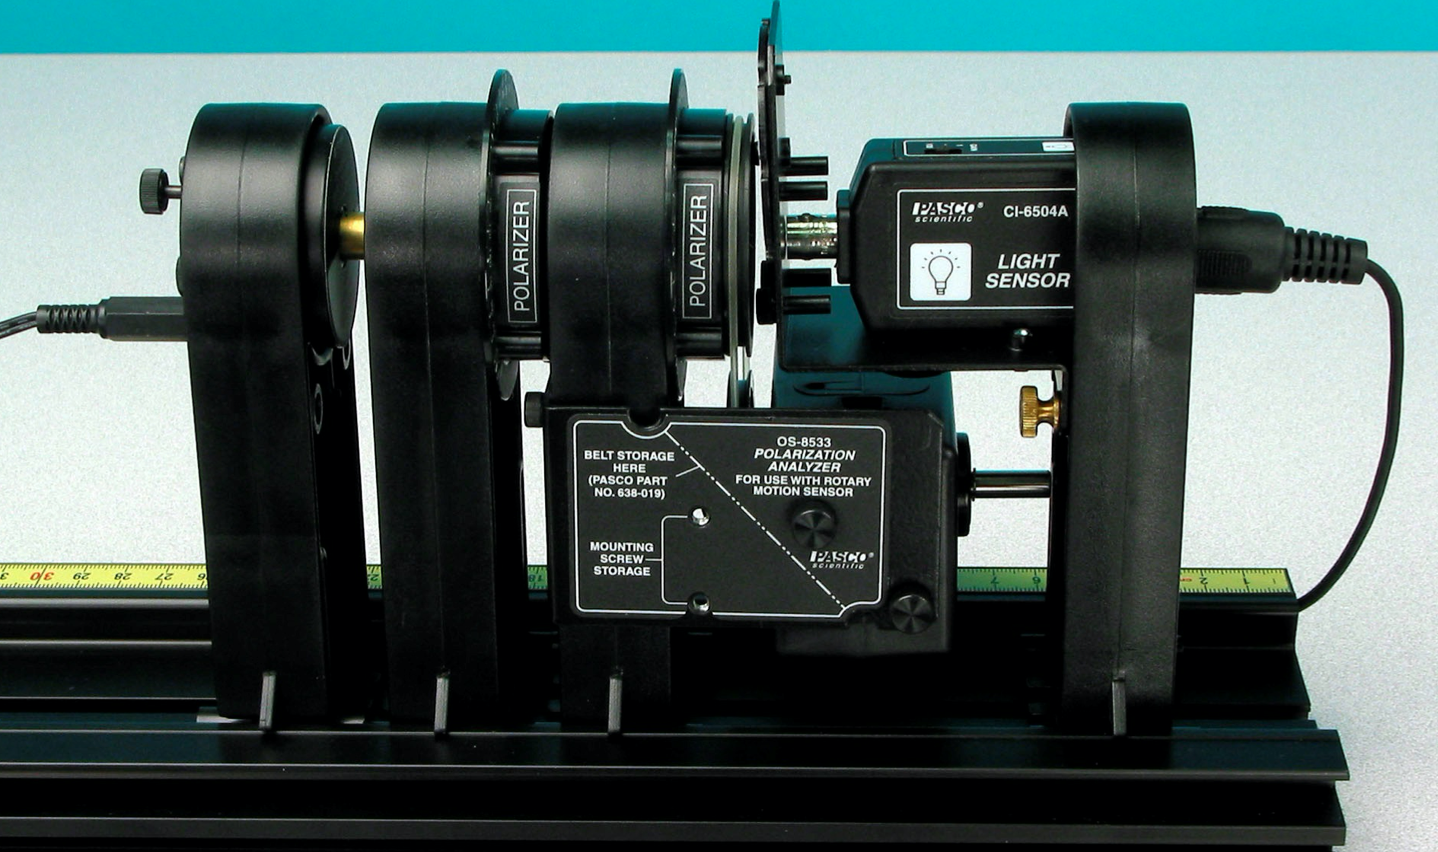
\includegraphics[width=9cm]{2 polarizers.png}
        \caption*{[Figure 2] Experimental setup and components of the two-polarizer apparatus. The apparatus consists of a laser diode, two polarizers, one of which is exporting data to LabView, and a diode detector.}
    \end{figure}

    Once a sufficient amount of data was collected for two polarizers, a third polarizer was added behind the acquisition lens, which was then removed to calibrate the second polarizer. This was done by adjusting the second polarizer so that its direction was orthogonal to that of the first polarizer, and a minimal amount of light was being detected in LabView. The acquisition polarizer was then re-added, and LabView was set to record $2\pi$ radians as the center polarizer was manually adjusted. Again, this experiment was repeated until the observed data was consistent, uniform, and smooth. The apparatus is depicted in Figure 3:

    \begin{figure}[H]
        \centering
        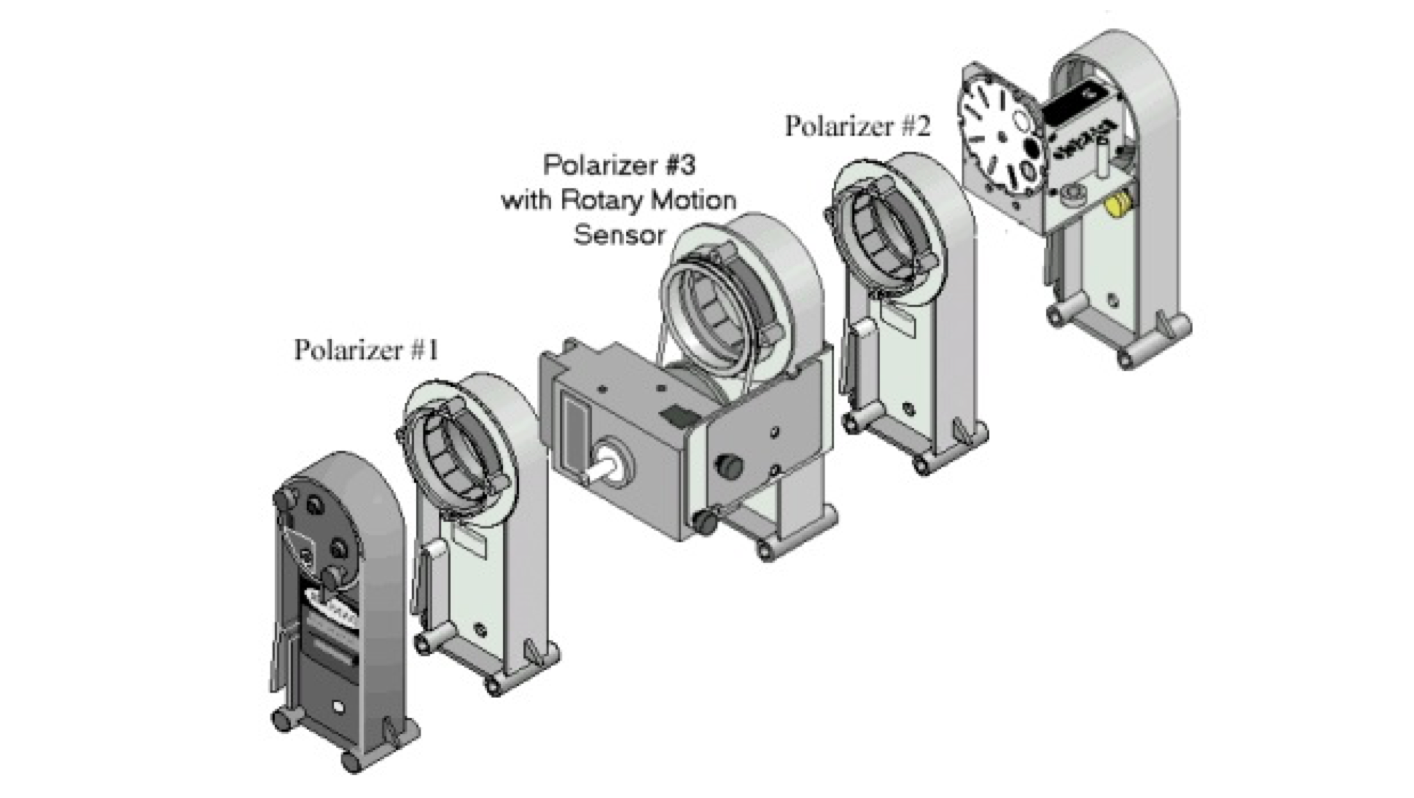
\includegraphics[width=9cm]{3 polarizers.png}
        \caption*{[Figure 3] Depiction of the experimental setup used in verifying Malus's law for three polarizers. The apparatus consists of three polarizers, one of which exports angle data to LabView, a laser diode, and detector.}
    \end{figure}

    The last set of trials which were performed were to determine Brewster's angle. The laser detector gain was configured to `10' and a collomating slit was placed in front to avoid over saturating the detector. The detector was attached to a long, rotatable arm. In the center of the rotator was an acryllic D-lens, which angle information was read by an acquisition device and exported to LabView. Incident to the D-lens was diode-laser light which had been polarized and run through a collomating slit to control the amount of light let through. The initial polarizer was the control, and was left in the horizontally-polarized position which was determined from the trials on Malus's law. The experimental apparatus is shown in Figure 4.

    \begin{figure}[H]
        \centering
        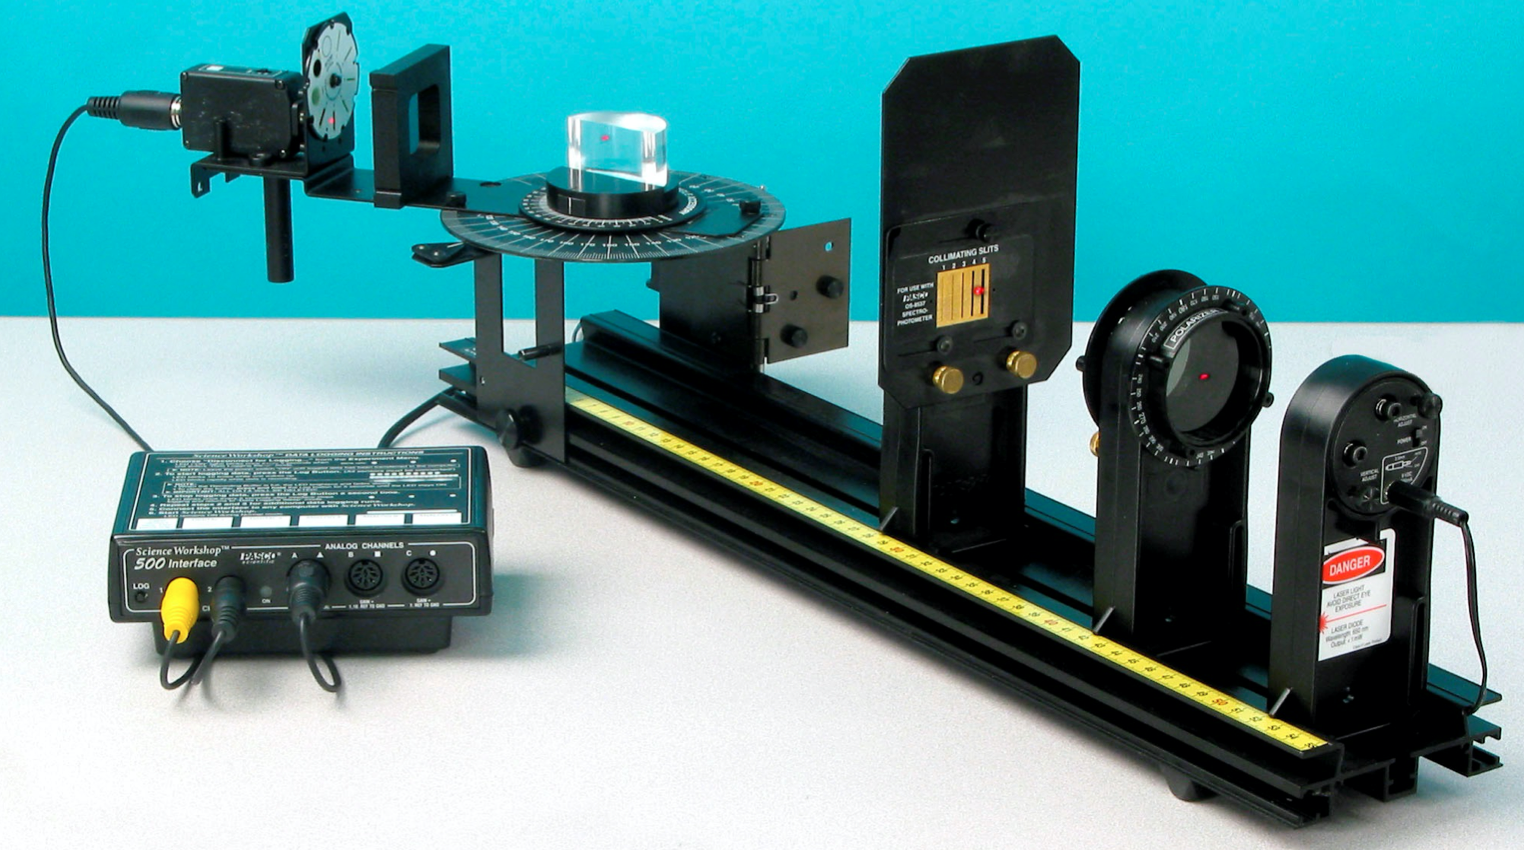
\includegraphics[width=9cm]{brewsty.png}
        \caption*{[Figure 4] Experimental setup for determining Brewester's angle. The apparatus consists of a rotatable D-lens, a laser diode, a polarizer, collomating slits and a detector.}
    \end{figure}



    

    \vspace{10pt}

    \fontfamily{qag} \selectfont \textbf{Data Analysis}
    
    \fontfamily{qpl} \selectfont 
    
    Following the form of the report, Malus's Law will be discussed first. The data, as recorded in \textit{Labview}, was stored in separate .txt files for each of the two trials (2 and 3 polaroids). 
    These files were read by the python library \textit{numpy}'s \textit{.readtxt()} function, and isolated by column for \textit{Intensity (V)} and \textit{position (radians)}.
    he raw data was plotted using another python library, \textit{matplotlib}, with uncertainties (see the upper charts of Figure N and Figure N+1 for the plots of the 2- and 3-polariod trials respectively).
    The uncertainties for each of these charts was one half of the smallest significant digit.
    The plot for 2-polarids was fit using an equation in the form of (6), and for 3-polaroids was fit using an equation in the form of (7) using \textit{scipy.optimize.curve\_fit()}. 
    Each of these functions had additional parameters for a phase-shift and an intensity offset.  

    The function fit the 3-polaroid trial quite easily, but the 2-polaroid trial was a little bit more tricky. The flatter tails at either end of the sinusoidal wave were culled from the dataset, and the function was able to fit (see Figure N to see the comparison between the original and culled data). 

    The results of these fits are discussed in the \textit{Results and Discussion section below}. The uncertainties of the relevant parameters of these fits (for these functions, $I_0$ and $I_1$ for the 2- and 3-polaroid trials respectively) were found by taking the square root of the covariance of the optimized parameters found by \textit{scipy.optimize.curve\_fit}. So long as the maximum value of the curve generated by these optimized parameters (as well as the majority of the curve itself) fit within the uncertainties of the measured data, the parameters are sufficient, within the uncertainty of the measurements. The residual plots of each trial (the difference between the fit curve and the measured data) were also plotted (the residual plots can be found in the lower charts of Figure N and Figure N+1).
    
    
    \vspace{10pt}

    \fontfamily{qag} \selectfont \textbf{Results and Discussion}
    
    \fontfamily{qpl} \selectfont 



    \vspace{10pt}

    \fontfamily{qag} \selectfont \textbf{Conclusions}
    
    \fontfamily{qpl} \selectfont 




\end{multicols}

    \vspace{10pt}
     
    \fontfamily{qag} \selectfont

    \begin{thebibliography}{}\fontfamily{qpl} \selectfont
        \bibitem{Item}\url{https://www.physics.utoronto.ca/~phy224_324/experiments/polarization-of-light/polar.pdf}
        \bibitem{Item}\url{https://www.ccmr.cornell.edu/wp-content/uploads/sites/2/2016/02/Refraction-Lab.pdf}=
        \bibitem{Item}\url{https://www.brown.edu/research/labs/mittleman/sites/brown.edu.research.labs.mittleman/files/uploads/lecture13_0.pdf}
        \bibitem{Item}\url{https://aip.scitation.org/doi/pdf/10.1063/1.4943751}
    \end{thebibliography}




    \pagebreak 



    \fontfamily{qag} \selectfont \textbf{Appendix I: Figures and Tables}
    
    \fontfamily{qpl} \selectfont

\begin{multicols}{2}
    \begin{figure}[H]
        \hspace{-25pt} 
        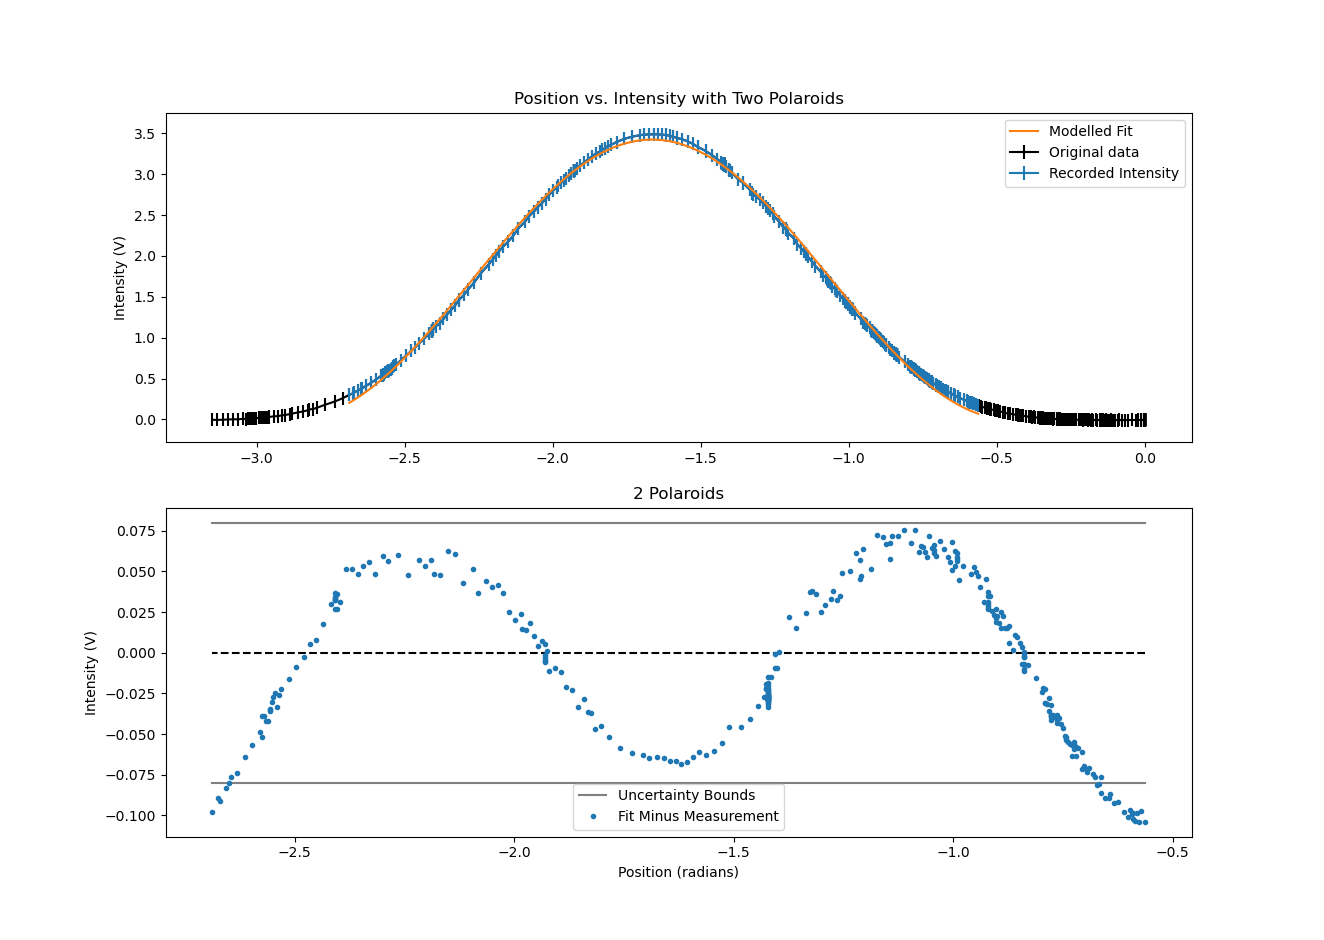
\includegraphics[width=3.7in]{malus_2.png}
        \caption{add later.}
        \label{fig:malus_2}
    \end{figure}

\vspace{-20pt}

    \begin{figure}[H]
        \hspace{-5pt}
        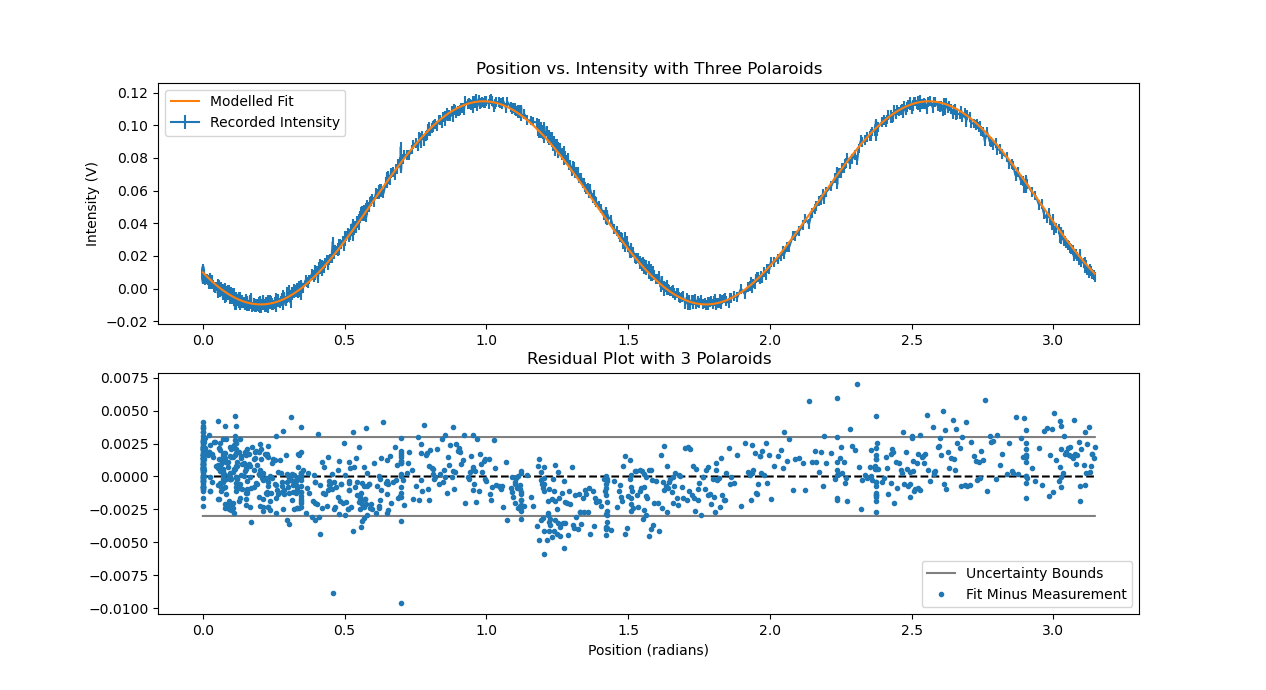
\includegraphics[width=3in]{malus_3.png}
        \caption{add later.}
        \label{fig:malus_3}
    \end{figure}

% \vspace{0pt}

%     \begin{figure}[H]
%         \centering 
%         \includegraphics[width=5.5in]{IMG_0450.jpg}
%         \caption*{[Figure 3] The plotted data for all three trials, including uncertainties and calibrated curve fits. (Above) Trial 1, at 60s intervals with initial temperature $27^\circ$C. (Middle) Trial 2, at 45s intervals with initial temperature $29^\circ$C. (Below) Trial 3, again at 60s interval but with initial temperature $97^\circ$C. }
%     \end{figure}

% \vspace{-20pt}

    % \begin{figure}[H]
    %     \centering 
    %     \includegraphics[width=7in]{uncertainty data.png}
    %     \caption*{[Figure 4] The visual overlap of the uncertainties recorded for acquired data and curve\_fit parameter covariances. The columns indicate trial number, while the rows indicate the `uncertainty of worst fit' (Left) and the distance between errors (Right). These plots were created by varying the optimal curve fit parameters with the maximum uncertainty of the covariances, and the comparing the uncertainty overlap with acquired data. }
    % \end{figure}


\end{multicols}





\end{document}